\section{Package syntax and semantics}
\label{sec:syntax}
This section contains a definition of the syntax and semantics of the PMF
package for \sbmlthreecore. The PMF package involves the following new object
classes:

\begin{itemize}
	\item \CompartmentMetaData
	\item \Correlation
	\item \DataSource
	\item \ListOfCorrelations
	\item \ListOfDataSources
	\item \ListOfModelVariables
	\item \ListOfPrimaryModels
	\item \ListOfReferences
	\item \ModelVariable
	\item \ParameterMetaData
	\item \PrimaryModel
	\item \Reference
	\item \RuleMetaData
	\item \SpeciesMetaData
	\item \UnitTransformation
\end{itemize}

\sec{examples} contains complete examples of using the constructs in SBML
models.

\subsection{Namespace URI and other declarations necessary for using this
			package}
\label{xml-namespace}

Every SBML Level~3 package is identified uniquely by an XML namespace URI. For
an SBML document to be able to use a given Level~3 package, it must declare the
use of that package by referencing its URI. The following is the namespace URI
for this version of the PMF package for \sbmlthreecore:
\begin{center}
\uri{http://www.sbml.org/sbml/level3/version1/pmf/version1}
\end{center}

In addition, SBML documents using a given packge must indicate whether the
package can be used to change the mathematical interpretation of a model. This
is done using the attribute \token{required} on the \token{<sbml>} element in
the SBML document. For the PMF package, the value of this attribute must be
\val{false}, because the use of the PMF package cannot change the mathematical
meaning of a model.

The following fragmen illustrates the beginning of a typical SBML model using
\sbmlthreecore and this version of the PMF package.

\begin{example}
<?xml version="1.0" encoding="UTF-8"?>
<sbml xmlns="http:/www.sbml.org/sbml/level3/version1/core" level="3" version="1"
	xmlns:pmf="http://www.sbml.org/sbml/level3/version1/pmf/version1"
	pmf:required="false">
\end{example}


\subsection{Primitive data types}
\label{new-primitive-types}
The PMF package includes a new primitve data type, the \primtype{ModelClass}.

\subsubsection{Type \fixttspace\primtypeNC{ModelClass}}
\label{primtype-modelclass}
The \primtype{ModelClass} primitive data type is used in the deefinition of the
\RuleMetaData class. \primtype{ModelClass} is derived from type
\primtype{string} and its values are restricted to being one of the
possibilities listed in \tab{primtype-modelclass-values}.

\begin{table}
	\begin{tabular}{|l|}
		\hline
		\val{unknown} \\ \hline
		\val{growth} \\ \hline
		\val{inactivation} \\ \hline
		\val{survival} \\ \hline
		\val{growth/inactivation} \\ \hline
		\val{inactivation/survival} \\ \hline
		\val{growth/survival} \\ \hline
		\val{growth/inactivation/survival} \\ \hline
		\val{T} \\ \hline
		\val{PH} \\ \hline
		\val{aw} \\ \hline
		\val{T/pH} \\ \hline
		\val{T/aw} \\ \hline
		\val{pH/aw} \\ \hline
		\val{T/pH/aw} \\ \hline
	\end{tabular}
	\caption{Possible values for \primtype{ModelClass}}
	\label{primtype-modelclass-values}
\end{table}

Attributes of type \primtype{ModelClass} cannot take on any other values. The
meaning of these values is discussed in the context of the \RuleMetaData class'
definition in \sec{rulemetadata-class}.

\subsection{Meta data classes}
The \Pmf package extends a number of classes from SBML Level 3 Version 1 with
the addition of meta data classes. These classes act as place holders for extra
meta data. The newly introduced meta data classes are:
\begin{itemize}
	\item \CompartmentMetaData
	\item \ParameterMetaData
	\item \RuleMetaData
	\item \SpeciesMetaData
\end{itemize}


\subsubsection{The \class{CompartmentMetaData} class}
\label{compartmentmetadata-class}
The \CompartmentMetaData further describes a Compartment with two attributes:
\token{source} and \token{detail}. \fig{compartment_uml} provides the UML
diagram of its definition.

\paragraph{The source attribute}
The optional attribute \token{source} contains a signed integer refering to the
PMF matrix vocabulary.

\paragraph{The detail attribute}
The optional attribute \token{detail} contains a string with extra details of
the \Compartment object.


\subsubsection{The \class{ParameterMetaData} class}
\label{parametermetadata-class}
The \ParameterMetaData further describes a Parameter with the optional
attributes: \token{p}, \token{t}, \token{error}, \token{description},
\token{min} and \token{max}. \fig{parameter_uml} provides the UML diagram of its
definition.

\paragraph{The \token{p} attribute}
The optional attribute \token{p} contains a \primtype{double} with the partition
coefficient (P) of the parameter.

\paragraph{The \token{t} attribute}
The optional attribute \token{t} contains a \primtype{double} with the
\emph{t-statistic} of the parameter.

\paragraph{The \token{error} attribute}
The optional attribute \token{error} contains a \primtype{double} with the
\emph{error} of the parameter.

\paragraph{The \token{description} attribute}
The optional attribute \token{description} contains a \primtype{string} with the
description of the parameter.

\paragraph{The \token{min} attribute}
The optional attribute \token{min} contains a \primtype{double} with the
minimum value of the parameter.

\paragraph{The \token{max} attribute}
The optional attribute \token{max} contains a \primtype{double} with the
maximum value of the parameter.

\fig{model_uml} features an example of \ParameterMetaData.


\subsubsection{The \class{RuleMetaData} class}
\label{rulemetadata-class}
The \RuleMetaData further describes a \Rule with the optional attributes:
\token{formulaName}, \token{pmmLabId} and \token{modelClass}. \fig{rule_uml}
provides the UML diagram of its definition.

\paragraph{The \token{formulaName} attribute}
The formulaName attribute

\paragraph{The \token{pmmLabId} attribute}
Optional attriubte of type \primtype{integer} with the PmmLab id.

\paragraph{The \token{modelClass} attribute}
Optional attribute of type ModelClass with the class of the model.


\subsubsection{The \class{SpeciesMetaData} class}
\label{speciesmetadata-class}
The \SpeciesMetaData further describes a \Species with the optional attributes:
\token{source}, \token{detail} and \token{description}. \fig{species_uml}
provides the UML diagram of its definition.

\paragraph{The \token{source} attribute}
Optional attribute of type \primtype{string} with the source of the species

\paragraph{The \token{detail} attribute}
Optional attribute of type \primtype{string} with the detail of the species

\paragraph{The \token{description} attribute}
Optional attribute of type \primtype{ModelClass} with the class of the model.

\begin{example}
<species compartment="Culture_medium" boundaryCondition="false" constant="false"
  id="some_species" hasOnlySubstanceUnits="true">
  <pmf:parameterMetaData xlmns:pmf="http://www.sbml.org/sbml3/version1/pmf/version1"
    description="bacterial population at time-ln()" detail="Salmonella spec"
    source="http://identifiers.org/ncim/C0036111" />
</species>
\end{example}


\subsection{New classes}
The \Pmf package also includes a number of new elements.
\begin{itemize}
	\item \Correlation
	\item \DataSource
	\item \ModelVariable
	\item \Reference
	\item \UnitTransformation
\end{itemize}

\subsubsection{The \class{Correlation} class}
\label{correlation-class}
The \Correlation expresses the existing dependence between the current\
\Parameter and a second \Parameter. It involves two attributes: \token{name}
and \token{value}. \fig{compartment_uml} provides its UML diagram.

\paragraph{The name attribute}
Mandatory attribute with the name of the second parameter.

\paragraph{The value attribute}
Mandatory attribute with the value of the dependence with the second parameter.

\subsubsection{The \class{DataSource} class}
\label{datasource-class}
The \DataSource is used to link to a separated file with numerical data
associated to the model. \fig{model_uml} provides its UML diagram.

\subsubsection{The \class{ModelVariable} class}
\label{modelvariable-class}
The \ModelVariable is used to describe a variable of the model such as
temperature, water activity, pH, etc. \fig{model_uml} provides its UML diagram.

\subsubsection{The \class{PrimaryModel} class}
\label{primarymodel-class}
The \PrimaryModel is used to link to a meta data file describing a primary model
with current model. \fig{model_uml} provides its UML diagram.

\subsubsection{The \class{Reference} class}
\label{reference-class}
The \Reference class is used to annotate a literature reference associated to
the model. It involves the following attributes. All the attributes of the
\Reference class are optional. The attributes are encoded using a subset of the
RIS specification format as described in \tab{reference-class-attributes}.

\begin{table}
	\begin{tabular}{|l|l|}
		\hline
		\textbf{Attribute} & \textbf{Description} \\
		\hline
		\token{AU} & String with the author\\
		\token{PY} & String with the publication year\\
		\token{TI} & String with the title.\\
		\token{AB} & String with the abstract.\\
		\token{T2} & String with the journal.\\
		\token{VL} & String with the volume.\\
		\token{IS} & String with the issue.\\
		\token{SP} & Integer with the page.\\
		\token{LB} & Integer with the approval mode.\\
		\token{UR} & String with the website.\\
		\token{M3} & String with the type of literature.\\
		\token{N1} & String with a comment.\\
		\hline
	\end{tabular}
	\caption{Attributes of the \Reference class}
	\label{reference-class-attributes}
\end{table}

\begin{example}
<pmf:reference
  xmlns:pmf="http://www.sbml.org/sbml/level3/version1/pmf/version"
  AU="Baranyi, J" PY="1995" TI="Mathematics of predictive food microbiology"
  AB="Commonly encountered problems related to ..." VL="26" IS="2" SP="199" />
\end{example}

\subsubsection{The \class{UnitTransformation} class}
\label{unittransformation-class}
The \UnitTransformation further describes a \UnitDefinition with the optional
attribute transformation, of type \primtype{string}, which holds the
transformation of the \UnitDefinition. \fig{unitdefinition_uml} provides the
UML diagram of its defintion. \fig{unitdefinition_uml} sports an example of
\UnitTransformation.

\subsection{New \ListOf classes}
The \Pmf package introduces new classes extending the \ListOf class. These
classes are derived from \SBase and inherit the attributes \token{metaid} and
\token{sboTerm}, as well as the subcomponents for \Annotation and \Notes. There
are not empty lists, the lists must contain at least one object. The list
contain only one type of object.

\begin{table}
	\begin{tabular}{|l|l|}
		\hline
		\textbf{\ListOf class} & \textbf{Contained class}\\
		\hline
		\ListOfCorrelations & \Correlation\\
		\ListOfDataSources & \DataSource\\
		\ListOfModelVariables & \ModelVariable\\
		\ListOfPrimaryModels & \PrimaryModel\\
		\ListOfReferences & \Reference\\
		\hline
	\end{tabular}
	\caption{New \ListOf classes}
	\label{listof-classes}
\end{table}


\subsection{Extended classes}
\begin{itemize}
	\item \Compartment
	\item \Model
	\item \Parameter
	\item \Rule
	\item \Species
	\item \UnitDefinition
\end{itemize}

\subsubsection{\class{Compartment}}
The \Compartment class is extended with one \CompartmentMetaData to hold extra
meta data related to the compartment. \fig{compartment_uml} provides the UML
diagram for the extension.

\begin{example}
<compartment id="Culture_medium" name="Culture medium" constant="true"
  <pmf:compartmentMetaData xmlns:pmf="http://www.sbml.org/sbml/level3/version1/pmf/version1"
    detail="broth" source="36">
</compartment>
\end{example}

\begin{figure}
	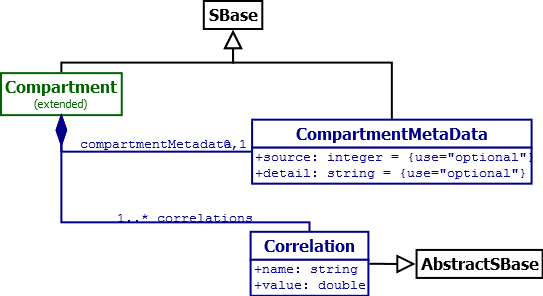
\includegraphics[scale=0.8]{img/compartment_uml}
	\caption{Class diagram of extended Compartment}
	\label{compartment_uml}
\end{figure}

\subsubsection{\class{Model}}
The \Model class is extended with the optional lists \ListOfPrimaryModels,
\ListOfDataSources and \ListOfPrimaryModels. \fig{model_uml} provides the UML
diagram for the extension.

\begin{example}
<model id="model">
  <pmf:listOfModelVariables xmlns:pmf="http://www.sbml.org/sbml/level3/version1/pmf/version1">
    <pmf:modelVariable name="pH" value="5.0" />
    <pmf:modelVariable name="T" value="20.0" />
  </pmf:listOfModelVariables>
  <pmf:listOfPrimaryModels xmlns:pmf="http://www.sbml.org/sbml/level3/version1/pmf/version1">
    <pmf:primaryModel src="someModel.sbml" />
  </pmf:listOfPrimaryModels>
  <pmf:listOfDataSources
    xlmns:pmf="xmlns:pmf="http://www.sbml.org/sbml/level3/version1/pmf/version1">
    <pmf:dataSource src="someData.numl" />
  </pmf:listOfDataSources>
</model>
\end{example}

\begin{figure}
	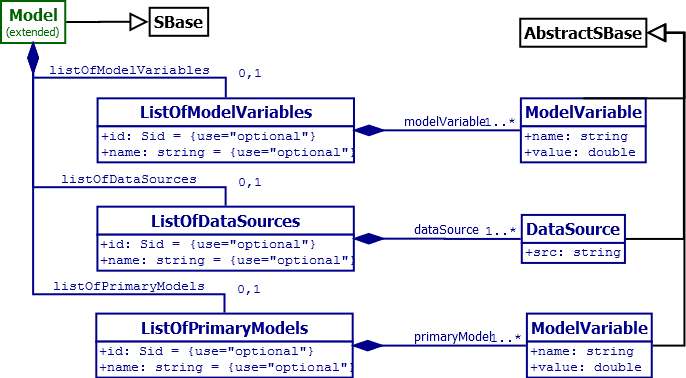
\includegraphics[scale=0.7]{img/model_uml}
	\caption{Class diagram of extended Model}
	\label{model_uml}
\end{figure}

\subsubsection{\class{Parameter}}
The \Parameter class is extended with one \ListOfCorrelations and one optional
\ParameterMetaData.

\begin{example}
<parameter constant="false" id="p" value="0">
  <pmf:parameterMetaData xmlns:pmf="http://www.sbml.org/sbml/level3/version1/pmf/version1">
  <pmf:listOfCorrelations xlmns:pmf="http://wwww.sbml.org/sbml/level3/version1/pmf/version1">
    <pmf:correlation name="a" value="1" />
    <pmf:correlation name="b" value="2" />
  </pmf:listOfCorrelations>
</parameter>
\end{example}

\begin{figure}
	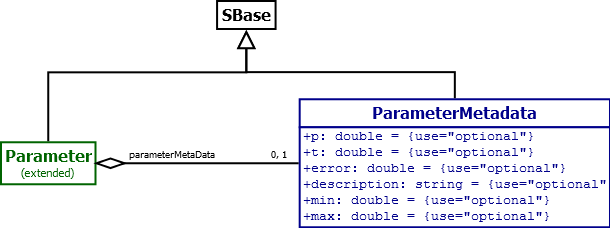
\includegraphics[scale=0.7]{img/parameter_uml}
	\caption{Class diagram of extended Parameter}
	\label{parameter_uml}
\end{figure}

\subsubsection{\class{Rule}}
The \Rule class is extended with a \ListOfReferences and one optional
\RuleMetaData.
\begin{example}
<algebraicRule>
  <math xmlns="http://www.w3.org/1998/Math/MathML">
    <plus/>
    <cn>2</cn>
    <cn>2</cn>
  </math>
  <pmf:ruleMetaData xmlns:pmf="https://www.sbml.org/sbml/level3/version1/pmf/version1"
    formulaName="2 plus 2" ruleClass="growth" pmmLabID="1" />
</algebraicRule>
\end{example}

\begin{figure}
	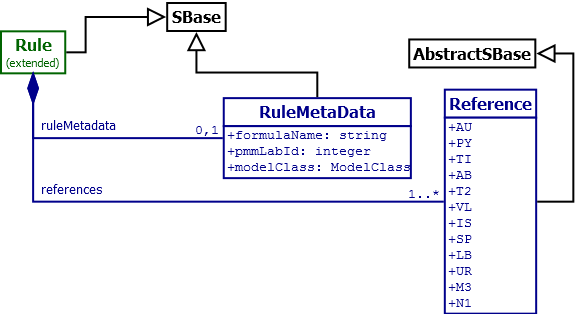
\includegraphics[scale=0.7]{img/rule_uml}
	\caption{Class diagram of extended Rule}
	\label{rule_uml}
\end{figure}

\subsubsection{\class{Species}}
The \Species class is extended with one optional \SpeciesMetaData.
\begin{example}
<species compartment="Culture_medium" boundaryCondition="false" constant="false"
  id="some_species" hasOnlySubstanceUnits="true">
  <pmf:speciesMetaData xmlns:pmf="http://www.sbml.org/sbml/level3/version1/pmf/version1"
    description="bacterial population at time t-ln()" detail="Salmonella spec"
    source="http://identifiers.org/ncim/C0036111" />
</species>
\end{example}

\begin{figure}
	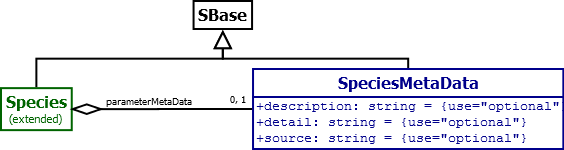
\includegraphics[scale=0.7]{img/species_uml}
	\caption{Class diagram of extended Species}
	\label{species_uml}
\end{figure}

\subsubsection{\class{UnitDefinition}}
The \UnitTransformation class is extended with an optional \UnitTransformation.

\begin{example}
<unitDefinition id="ln_count_g" name="ln(count/g)">
  <pmf:unitTransformation xmlns:pmf="http://www.sbml.org/sbml/level3/version1/pmf/version1"
    name="ln" />
</unitDefinition>
\end{example}

\begin{figure}
	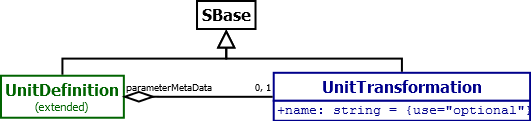
\includegraphics[scale=0.7]{img/unitdefinition_uml}
	\caption{Class diagram of extended UnitDefinition}
	\label{unitdefinition_uml}
\end{figure}
